\documentclass{standalone}
\usepackage{tikz}
\usetikzlibrary{patterns, positioning}

\begin{document}
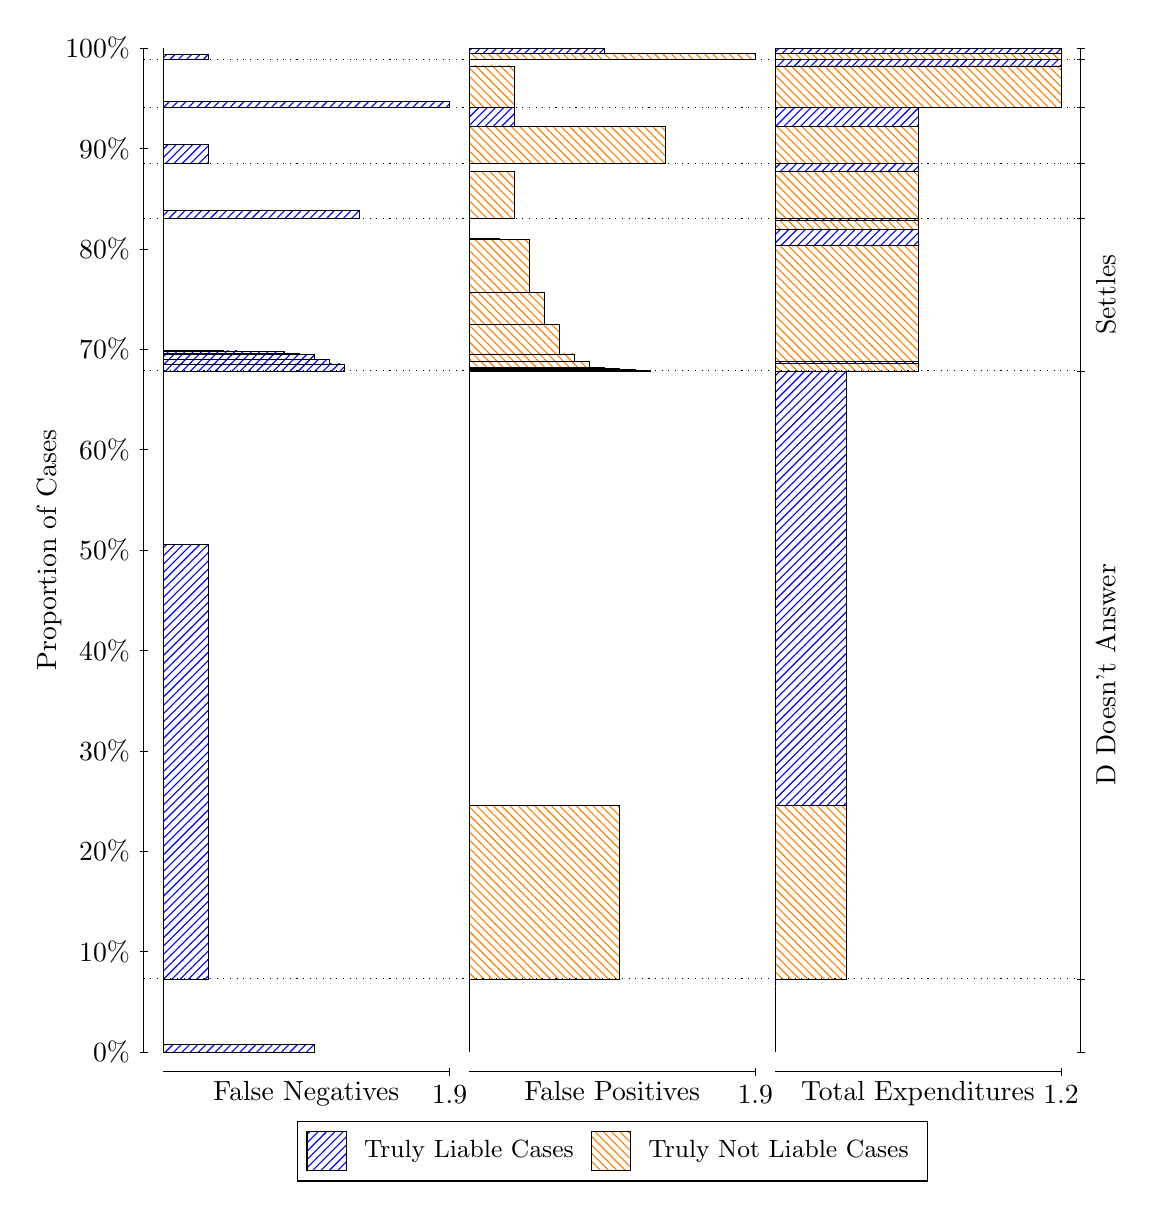
\begin{tikzpicture}
\draw[black, very thin] (1.5,1.75) -- (1.5,14.5);
\node[rotate=90, anchor=center] at (0.3, 8.125) {Proportion of Cases};
\draw[black, very thin] (1.45,1.75) -- (1.55,1.75);
\node[anchor=east] at (1.45, 1.75) {0\%};
\draw[black, very thin] (1.45,3.025) -- (1.55,3.025);
\node[anchor=east] at (1.45, 3.025) {10\%};
\draw[black, very thin] (1.45,4.3) -- (1.55,4.3);
\node[anchor=east] at (1.45, 4.3) {20\%};
\draw[black, very thin] (1.45,5.575) -- (1.55,5.575);
\node[anchor=east] at (1.45, 5.575) {30\%};
\draw[black, very thin] (1.45,6.85) -- (1.55,6.85);
\node[anchor=east] at (1.45, 6.85) {40\%};
\draw[black, very thin] (1.45,8.125) -- (1.55,8.125);
\node[anchor=east] at (1.45, 8.125) {50\%};
\draw[black, very thin] (1.45,9.4) -- (1.55,9.4);
\node[anchor=east] at (1.45, 9.4) {60\%};
\draw[black, very thin] (1.45,10.675) -- (1.55,10.675);
\node[anchor=east] at (1.45, 10.675) {70\%};
\draw[black, very thin] (1.45,11.95) -- (1.55,11.95);
\node[anchor=east] at (1.45, 11.95) {80\%};
\draw[black, very thin] (1.45,13.225) -- (1.55,13.225);
\node[anchor=east] at (1.45, 13.225) {90\%};
\draw[black, very thin] (1.45,14.5) -- (1.55,14.5);
\node[anchor=east] at (1.45, 14.5) {100\%};

\draw[black, very thin] (13.4,1.75) -- (13.4,14.5);
\draw[black, very thin] (13.35,1.75) -- (13.45,1.75);
\node[anchor=west] at (13.35, 1.75) {};
\draw[black, very thin] (13.35,2.6778) -- (13.45,2.6778);
\node[anchor=west] at (13.35, 2.6778) {};
\draw[black, very thin] (13.35,10.399) -- (13.45,10.399);
\node[anchor=west] at (13.35, 10.399) {};
\draw[black, very thin] (13.35,12.334) -- (13.45,12.334);
\node[anchor=west] at (13.35, 12.334) {};
\draw[black, very thin] (13.35,13.037) -- (13.45,13.037);
\node[anchor=west] at (13.35, 13.037) {};
\draw[black, very thin] (13.35,13.745) -- (13.45,13.745);
\node[anchor=west] at (13.35, 13.745) {};
\draw[black, very thin] (13.35,14.354) -- (13.45,14.354);
\node[anchor=west] at (13.35, 14.354) {};
\draw[black, very thin] (13.35,14.5) -- (13.45,14.5);
\node[anchor=west] at (13.35, 14.5) {};

\draw[black, very thin, pattern color=blue, pattern=north east lines] (1.75,1.75) rectangle (3.6623,1.8476);
\draw[black, very thin, pattern color=orange, pattern=north west lines] (1.75,1.8476) rectangle (1.75,2.6778);
\draw[black, very thin, pattern color=blue, pattern=north east lines] (1.75,2.6778) rectangle (2.3237,8.1978);
\draw[black, very thin, pattern color=orange, pattern=north west lines] (1.75,8.1978) rectangle (1.75,10.399);
\draw[black, very thin, pattern color=blue, pattern=north east lines] (1.75,10.399) rectangle (4.0447,10.488);
\draw[black, very thin, pattern color=blue, pattern=north east lines] (1.75,10.488) rectangle (3.8535,10.548);
\draw[black, very thin, pattern color=blue, pattern=north east lines] (1.75,10.548) rectangle (3.6623,10.607);
\draw[black, very thin, pattern color=blue, pattern=north east lines] (1.75,10.607) rectangle (3.4711,10.61);
\draw[black, very thin, pattern color=blue, pattern=north east lines] (1.75,10.61) rectangle (3.4711,10.625);
\draw[black, very thin, pattern color=blue, pattern=north east lines] (1.75,10.625) rectangle (3.2798,10.643);
\draw[black, very thin, pattern color=blue, pattern=north east lines] (1.75,10.643) rectangle (3.0886,10.647);
\draw[black, very thin, pattern color=blue, pattern=north east lines] (1.75,10.647) rectangle (2.8974,10.651);
\draw[black, very thin, pattern color=blue, pattern=north east lines] (1.75,10.651) rectangle (2.7061,10.654);
\draw[black, very thin, pattern color=blue, pattern=north east lines] (1.75,10.654) rectangle (2.5149,10.662);
\draw[black, very thin, pattern color=orange, pattern=north west lines] (1.75,10.662) rectangle (1.75,12.334);
\draw[black, very thin, pattern color=blue, pattern=north east lines] (1.75,12.334) rectangle (4.236,12.437);
\draw[black, very thin, pattern color=orange, pattern=north west lines] (1.75,12.437) rectangle (1.75,13.037);
\draw[black, very thin, pattern color=blue, pattern=north east lines] (1.75,13.037) rectangle (2.3237,13.28);
\draw[black, very thin, pattern color=orange, pattern=north west lines] (1.75,13.28) rectangle (1.75,13.745);
\draw[black, very thin, pattern color=blue, pattern=north east lines] (1.75,13.745) rectangle (5.3833,13.827);
\draw[black, very thin, pattern color=orange, pattern=north west lines] (1.75,13.827) rectangle (1.75,14.354);
\draw[black, very thin, pattern color=blue, pattern=north east lines] (1.75,14.354) rectangle (2.3237,14.42);
\draw[black, very thin, pattern color=orange, pattern=north west lines] (1.75,14.42) rectangle (1.75,14.5);
\draw[black, very thin, pattern color=orange, pattern=north west lines] (5.6333,1.75) rectangle (5.6333,2.5802);
\draw[black, very thin, pattern color=blue, pattern=north east lines] (5.6333,2.5802) rectangle (5.6333,2.6778);
\draw[black, very thin, pattern color=orange, pattern=north west lines] (5.6333,2.6778) rectangle (7.5456,4.879);
\draw[black, very thin, pattern color=blue, pattern=north east lines] (5.6333,4.879) rectangle (5.6333,10.399);
\draw[black, very thin, pattern color=orange, pattern=north west lines] (5.6333,10.399) rectangle (7.9281,10.41);
\draw[black, very thin, pattern color=orange, pattern=north west lines] (5.6333,10.41) rectangle (7.7368,10.419);
\draw[black, very thin, pattern color=orange, pattern=north west lines] (5.6333,10.419) rectangle (7.5456,10.432);
\draw[black, very thin, pattern color=orange, pattern=north west lines] (5.6333,10.432) rectangle (7.3544,10.448);
\draw[black, very thin, pattern color=orange, pattern=north west lines] (5.6333,10.448) rectangle (7.1632,10.522);
\draw[black, very thin, pattern color=orange, pattern=north west lines] (5.6333,10.522) rectangle (6.9719,10.615);
\draw[black, very thin, pattern color=orange, pattern=north west lines] (5.6333,10.615) rectangle (6.7807,10.988);
\draw[black, very thin, pattern color=orange, pattern=north west lines] (5.6333,10.988) rectangle (6.5895,11.399);
\draw[black, very thin, pattern color=orange, pattern=north west lines] (5.6333,11.399) rectangle (6.3982,12.071);
\draw[black, very thin, pattern color=blue, pattern=north east lines] (5.6333,12.071) rectangle (6.0158,12.079);
\draw[black, very thin, pattern color=blue, pattern=north east lines] (5.6333,12.079) rectangle (5.8246,12.082);
\draw[black, very thin, pattern color=blue, pattern=north east lines] (5.6333,12.082) rectangle (5.6333,12.334);
\draw[black, very thin, pattern color=orange, pattern=north west lines] (5.6333,12.334) rectangle (6.207,12.935);
\draw[black, very thin, pattern color=blue, pattern=north east lines] (5.6333,12.935) rectangle (5.6333,13.037);
\draw[black, very thin, pattern color=orange, pattern=north west lines] (5.6333,13.037) rectangle (8.1193,13.502);
\draw[black, very thin, pattern color=blue, pattern=north east lines] (5.6333,13.502) rectangle (6.207,13.745);
\draw[black, very thin, pattern color=orange, pattern=north west lines] (5.6333,13.745) rectangle (6.207,14.272);
\draw[black, very thin, pattern color=blue, pattern=north east lines] (5.6333,14.272) rectangle (5.6333,14.354);
\draw[black, very thin, pattern color=orange, pattern=north west lines] (5.6333,14.354) rectangle (9.2667,14.434);
\draw[black, very thin, pattern color=blue, pattern=north east lines] (5.6333,14.434) rectangle (7.3544,14.5);
\draw[black, very thin, pattern color=orange, pattern=north west lines] (9.5167,1.75) rectangle (9.5167,2.5802);
\draw[black, very thin, pattern color=blue, pattern=north east lines] (9.5167,2.5802) rectangle (9.5167,2.6778);
\draw[black, very thin, pattern color=orange, pattern=north west lines] (9.5167,2.6778) rectangle (10.425,4.879);
\draw[black, very thin, pattern color=blue, pattern=north east lines] (9.5167,4.879) rectangle (10.425,10.399);
\draw[black, very thin, pattern color=orange, pattern=north west lines] (9.5167,10.399) rectangle (11.333,10.495);
\draw[black, very thin, pattern color=blue, pattern=north east lines] (9.5167,10.495) rectangle (11.333,10.521);
\draw[black, very thin, pattern color=orange, pattern=north west lines] (9.5167,10.521) rectangle (11.333,11.99);
\draw[black, very thin, pattern color=blue, pattern=north east lines] (9.5167,11.99) rectangle (11.333,12.201);
\draw[black, very thin, pattern color=orange, pattern=north west lines] (9.5167,12.201) rectangle (11.333,12.307);
\draw[black, very thin, pattern color=blue, pattern=north east lines] (9.5167,12.307) rectangle (11.333,12.334);
\draw[black, very thin, pattern color=orange, pattern=north west lines] (9.5167,12.334) rectangle (11.333,12.935);
\draw[black, very thin, pattern color=blue, pattern=north east lines] (9.5167,12.935) rectangle (11.333,13.037);
\draw[black, very thin, pattern color=orange, pattern=north west lines] (9.5167,13.037) rectangle (11.333,13.502);
\draw[black, very thin, pattern color=blue, pattern=north east lines] (9.5167,13.502) rectangle (11.333,13.745);
\draw[black, very thin, pattern color=orange, pattern=north west lines] (9.5167,13.745) rectangle (13.15,14.272);
\draw[black, very thin, pattern color=blue, pattern=north east lines] (9.5167,14.272) rectangle (13.15,14.354);
\draw[black, very thin, pattern color=orange, pattern=north west lines] (9.5167,14.354) rectangle (13.15,14.434);
\draw[black, very thin, pattern color=blue, pattern=north east lines] (9.5167,14.434) rectangle (13.15,14.5);
\draw[black, dotted] (1.5,2.6778) -- (13.4,2.6778);
\draw[black, dotted] (1.5,10.399) -- (13.4,10.399);
\draw[black, dotted] (1.5,12.334) -- (13.4,12.334);
\draw[black, dotted] (1.5,13.037) -- (13.4,13.037);
\draw[black, dotted] (1.5,13.745) -- (13.4,13.745);
\draw[black, dotted] (1.5,14.354) -- (13.4,14.354);
\draw[black, very thin] (1.75,1.5) -- (5.3833,1.5);
\node[anchor=north] at (3.5667, 1.5) {False Negatives};
\draw[black, very thin] (5.3833,1.45) -- (5.3833,1.55);
\node[anchor=north] at (5.3833, 1.45) {1.9};

\draw[black, very thin] (5.6333,1.5) -- (9.2667,1.5);
\node[anchor=north] at (7.45, 1.5) {False Positives};
\draw[black, very thin] (9.2667,1.45) -- (9.2667,1.55);
\node[anchor=north] at (9.2667, 1.45) {1.9};

\draw[black, very thin] (9.5167,1.5) -- (13.15,1.5);
\node[anchor=north] at (11.333, 1.5) {Total Expenditures};
\draw[black, very thin] (13.15,1.45) -- (13.15,1.55);
\node[anchor=north] at (13.15, 1.45) {1.2};


\node[black, centered, rotate=90] at (13.72, 6.5384) {D Doesn't Answer};
\node[black, centered, rotate=90] at (13.72, 11.366) {Settles};





\draw (7.449999999999999,1.5) node[draw=none] (baseCoordinate) {};
\begin{scope}[align=center]
        \matrix[scale=0.5, draw=black, below=0.5cm of baseCoordinate, nodes={draw}, column sep=0.1cm]{
            \node[rectangle, draw, minimum width=0.5cm, minimum height=0.5cm, pattern=north east lines, pattern color=blue] {}; &
            \node[draw=none, font=\small] (B) {Truly Liable Cases}; &
            \node[rectangle, draw, minimum width=0.5cm, minimum height=0.5cm, pattern=north west lines, pattern color=orange] {}; &
            \node[draw=none, font=\small] (B) {Truly Not Liable Cases}; \\
            };
\end{scope}

\end{tikzpicture}
\end{document}